\section{Introduction}
\label{sec:intro}

A looped, or recurrent-depth, transformer applies one block of layers several times in a row
\citep{dehghani2019universal,geiping2025scaling,zhu2025scaling}. Running a block $r$ times costs $r$ times its
compute and adds no parameters. Two benefits are expected in return. The first is \emph{parameter efficiency}: a
looped model should behave like a larger dense model, which matters wherever memory or bandwidth rather than
arithmetic limits deployment. The second is \emph{latent reasoning}: if the loop iterates on a problem, running more
loops at inference should solve harder problems without writing out a chain of thought, a form of test-time compute
that lives inside the network.

Both claims are hard to check from the literature. Studies differ in data, tokenizer, training recipe and model
family; seeds are rarely reported; and the quantity of interest, how much one more loop is worth, is usually read off
a single fitted scaling law \citep{schwethelm2026how,prairie2026parcae,chen2026moe}. Evidence for test-time scaling
comes from two directions that are seldom put side by side: large models trained with a random number of loops, which
become robust to the loop count \citep{geiping2025scaling}, and small models on algorithmic tasks, which solve longer
problems when run longer \citep{fan2025looped,kohli2026loop,zhang2026recurrence}.

We measured both claims in one study, with one architecture family and one recipe, and with the hypotheses and the
analysis written down before the first training run. On web text, a grid of 111 runs varies model size (10M to 80M
looped, dense references to 160M), where the loop sits (a middle block or the whole stack), how often it runs ($r$ =
2, 4, 8) and how it is backpropagated (through all loops or through the last half), with three seeds at the small
sizes and cooldown branches at three data budgets. Extensions add a 160M looped model, up to 160 training tokens per
parameter, random loop counts, and nine supplementary experiments whose plans were frozen before they ran. When the
text results left the second claim untested, we built a task that needs serial steps, a chain of lookups in fixed
random tables, froze its design and predictions, and ran it the same way: looped models against dense models of equal
parameters and of equal executed depth, against a dense model that writes the chain out, and against pause tokens.

\begin{figure}[t]
  \centering
  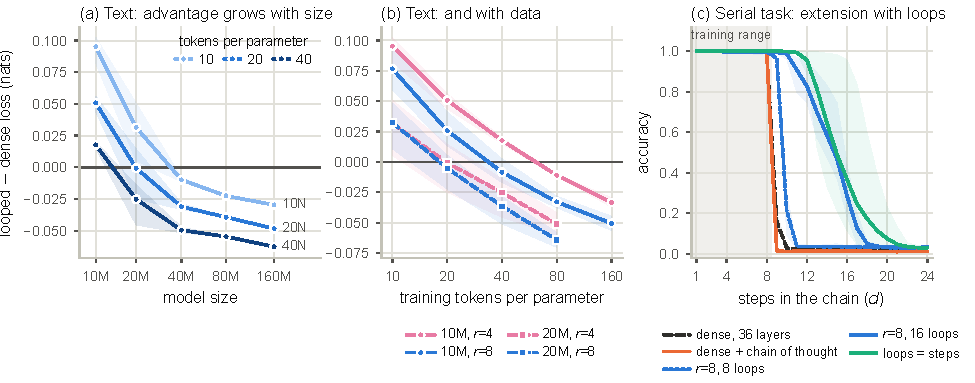
\includegraphics[width=\linewidth]{fig1_overview}
  \caption{What a loop buys, in one figure. \textbf{(a)}~On web text, at equal parameters and training tokens, a
  middle block looped 4 times goes from worse than the dense model at 10M to better at every budget from 40M on
  (looped minus dense validation loss; budgets of 10, 20 and 40 training tokens per parameter; band: range over
  seeds). \textbf{(b)}~The advantage also grows with the training tokens per parameter, here at 10M and 20M for
  middle blocks looped 4 and 8 times. \textbf{(c)}~On chains of table lookups, trained on 1--8 steps (shaded), dense
  models of the same executed depth stop at the training range, and so does a dense model that writes the chain out,
  whose prompt grows with the chain; a looped model run with more loops than in training solves longer chains (mean over
  five seeds; band: range).}
  \label{fig:overview}
\end{figure}

The two settings give different answers (Figure~\ref{fig:overview}). On text, the loop buys parameter and data
efficiency, not compute efficiency: measured without a fitted law, a parameter of the looped block is worth at most
about one dense parameter at 10--20M with up to 20 training tokens per parameter and about 1.3--1.5 dense parameters
at 40M--160M, the value grows with the tokens per parameter, and at equal training compute the dense model wins every
comparison we could measure, by a margin that shrinks with data. Depending on how it is trained, the looped block
runs a fixed-length program, a cycle or a fixed point, and none of these gains from extra loops at inference. On the
chain task, the same architecture computes the chain step by step inside the loop, solves chains longer than it was
trained on when run longer, and for most training regimes can tell from its own confidence when to stop. A written
chain of thought is perfect within the training range at a third of the compute and does not extend at all; on this
task, whose prompt grows with the chain, that is a failure to generalise to longer inputs.

We read the difference as a matter of three conditions, which the chain task meets once the model is trained for
them: \emph{headroom}, meaning that errors come from too few serial steps rather than from missing knowledge;
\emph{extendable iteration}, meaning that the loop can run longer without destroying its state; and a \emph{stopping
signal}. On web text at these sizes we saw no sign of the first. This reading is an interpretation of two settings,
not a tested law, and Section~\ref{sec:discussion} discusses what would test it.

Our contributions are:
\begin{itemize}
  \item \textbf{A pre-registered measurement of what a loop is worth on text} (Section~\ref{sec:text}). None of the four
  hypotheses held as stated. The pre-registered exponent $\varphi$ of the effective-parameter law
  $\Neff = \Nonce + r^{\varphi}\Nrec$ is not identified, because the dense law it is read from is weakly identified.
  Measured without that law, the value of a loop depends on model size and on training tokens per parameter, an
  interaction that effective-parameter laws with one exponent per architecture do not capture. At equal training
  compute the dense model wins all 258 measured comparisons, up to 640 tokens per parameter, and the two reach parity
  only at the smallest size and the most data, with the looped model's own learning rate.
  \item \textbf{What the looped block computes on text} (Section~\ref{sec:mechanism}). Depending on training, it runs
  a fixed-length program, a periodic cycle or a contraction to a fixed point; none gains from extra loops.
  \item \textbf{Loops as extendable depth on a serial task} (Section~\ref{sec:serial}). With dense controls of equal
  executed depth and probes of every intermediate value, looped models compute the chain step by step (one step per
  loop when the model has a loop for every step) and solve longer chains with more loops at inference.
  The learning rate decides whether this is learned at all. In a controlled comparison of answer-free stopping rules,
  the model's own confidence is the best rule that actually stops, and a training regime with a few random extra loops
  gives a model that both extends and stops.
  \item \textbf{A comparison with reasoning written out} (Section~\ref{sec:cot}). On this task, a dense model that
  writes the chain out as tokens is perfect within the training range and fails beyond it from the first written token
  on, a failure to generalise to longer prompts that leaves open what happens when the input length is fixed. Pause
  tokens add nothing.
  \item \textbf{The cost at deployment} (Section~\ref{sec:cost}), and an open record: the pre-registration, a dated log
  of every deviation and correction, and the results and training logs of all 232 language-model runs and 135
  synthetic-task runs (Section~\ref{sec:process}).
\end{itemize}
